\chapter{Конструкторский раздел}
В данном разделе представлены требования к программному обеспечению, рассмотрены структуры данных, алгоритмы и математические уравнения, выбранные для построения сцены.

\section{Требования к программному обеспечению}
Программное обеспечение должно обеспечивать следующую функциональность:
\begin{itemize}
    \item[---] Возможность ввода пользователем кривой и выбора оси вращения;
    \item[---] Вывод полученного тела вращения;
    \item[---] Возможность наложения фактуры или текстуры на тело по запросу пользователя;
    \item[---] Возможность изменения положения камеры в пространстве для обзора объекта под разными углами;
    \item[---] Освещение объекта статическим источником света.
\end{itemize}

\section{Используемые структуры данных}
Для реализации работы программы разработаны следующие структуры данных:
\begin{enumerate}
    \item Сцена содержит:
    \begin{itemize}
        \item[---] Тело вращения;
        \item[---] Источник света.
    \end{itemize}
    \item Тело вращения состоит из:
    \begin{itemize}
        \item[---] Массива вершин;
        \item[---] Массива граней;
        \item[---] Цвета тела вращения;
        \item[---] Нормалей точек.
    \end{itemize}
    \item Вершина объекта содержит:
    \begin{itemize}
        \item[---] Положение вершины в пространстве.
    \end{itemize}
    \item Грань объекта содержит: 
    \begin{itemize}
        \item[---] Индексы трех вершин из списка вершин тела вращения, образующих грань.
    \end{itemize}
    \item Источник света содержит:
    \begin{itemize}
        \item[---] Вектор направления источника;
        \item[---] Интенсивность источника.
    \end{itemize}
\end{enumerate}

\section{Алгоритм построения изображения}
Алгоритм генерации изображения представлен в виде диаграммы, оформленной в соответствии с нотацией IDEF0 и отражающей общую декомпозицию алгоритма:
\begin{figure}[H]
	\centering
	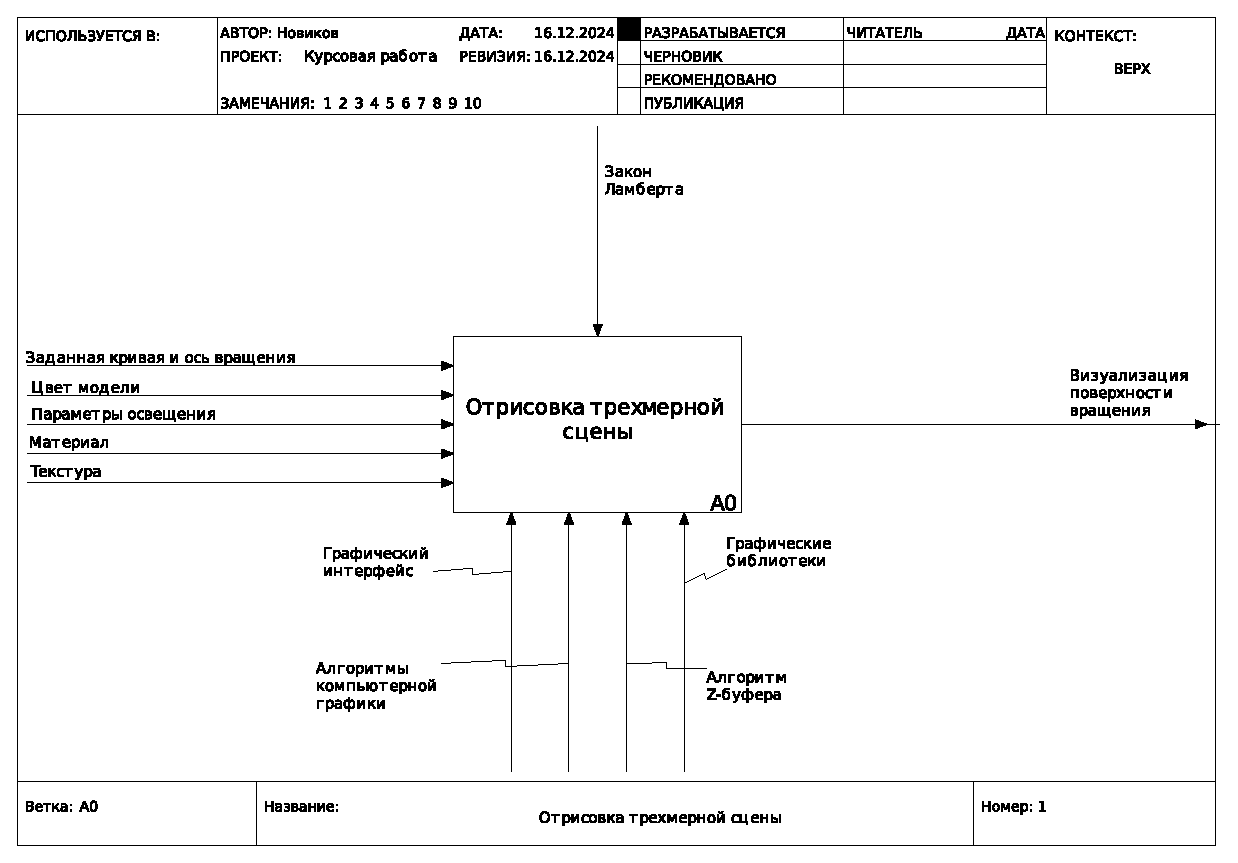
\includegraphics[scale=0.8]{img/01_A0.eps}
	\caption{Контекстная диаграмма верхнего уровня в нотации IDEF0}
	\label{fig:viewer}
\end{figure}

\begin{figure}[H]
	\centering
	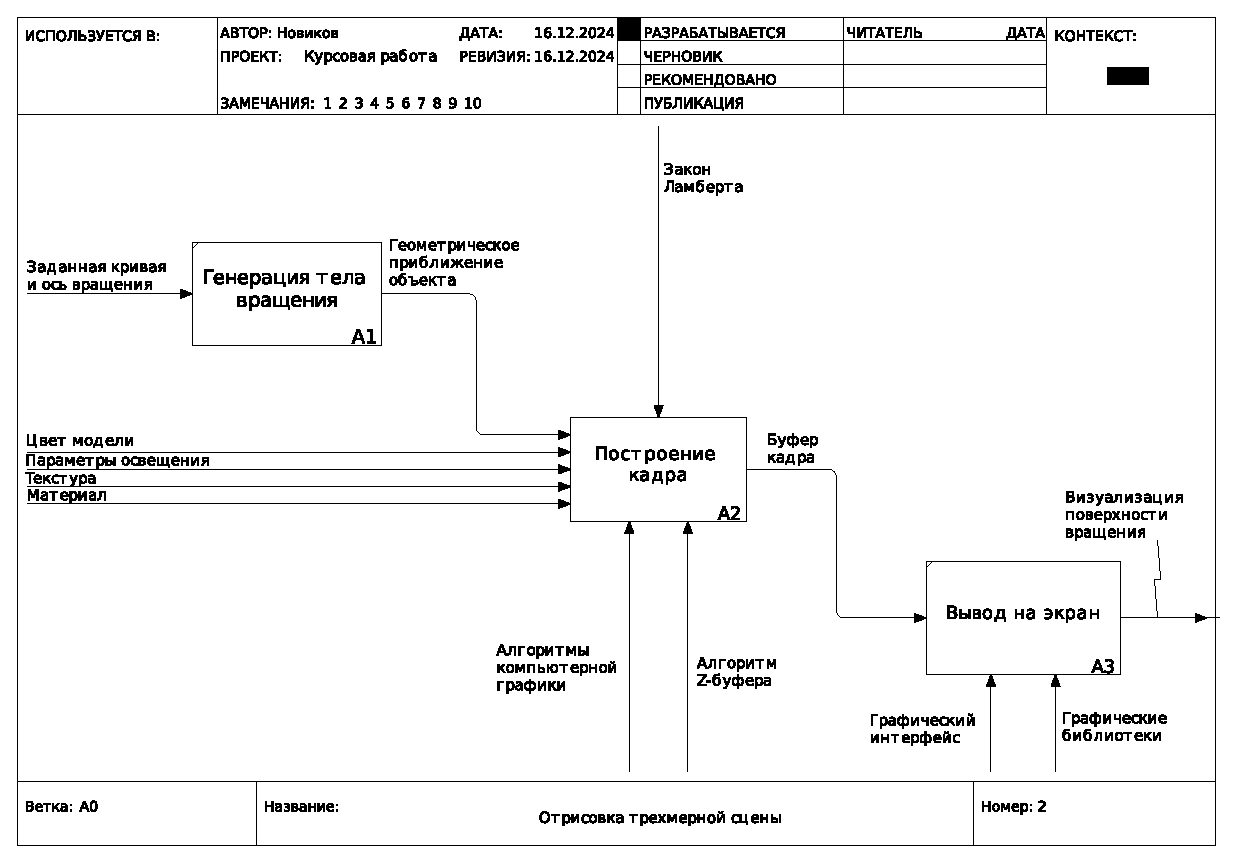
\includegraphics[scale=0.8]{img/02_A0.eps}
	\caption{Основной цикл ПО в нотации IDEF0}
	\label{fig:viewer}
\end{figure}

\begin{figure}[H]
	\centering
	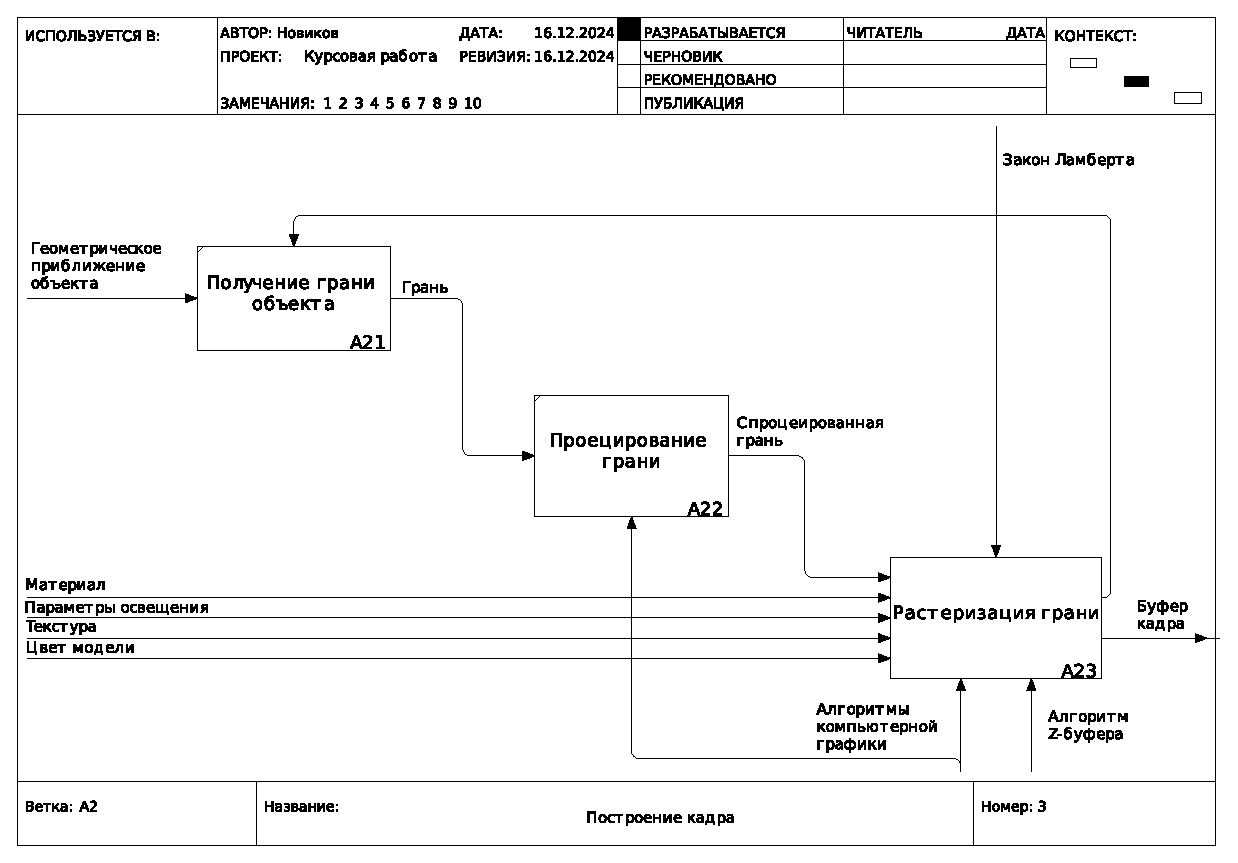
\includegraphics[scale=0.8]{img/03_A2.eps}
	\caption{Построение кадра в нотации IDEF0}
	\label{fig:viewer}
\end{figure}

\begin{figure}[H]
	\centering
	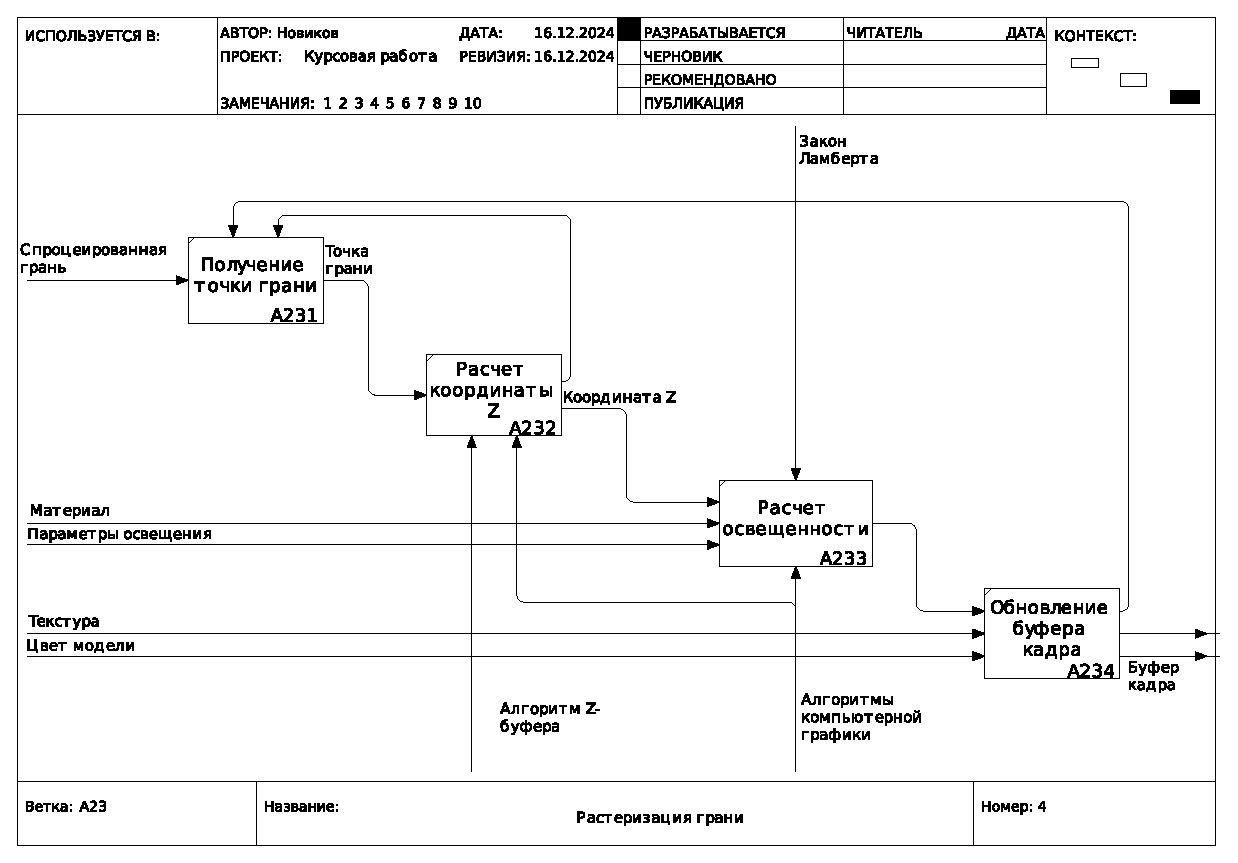
\includegraphics[scale=0.8]{img/04_A23.eps}
	\caption{Растерицазция грани в нотации IDEF0}
	\label{fig:viewer}
\end{figure}

\section{Алгоритм построения кривой}
Для построения кривой Безье по заданным точкам $P_1, P_2,..., P_n$, где $P_1, P_n$ --- начальная и конечная точки, $P_2, P_3, ..., P_{n-1}$ --- необязательные контрольные точки, задающие форму кривой, используется алгоритм де Кастельжо. Для заданных контрольных точек итеративно вычисляются новые промежуточные точки, для этого отрезки $P_1P_2, P_2P_3,...,P_{n-1}P_n$ разделяются в отношении $\frac{t}{1-t}$, где $t\in[0,1]$. Разбиение продолжается до тех пор, пока не останется одна точка, которая будет являться точкой кривой для заданного параметра $t$.

\section{Алгоритм построения тела вращения}
Для построения тела вращения для каждой точки кривой $C = (P_1, P_2,...,P_n)$ необходимо вычислить соответствующие точки на поверхности, полученные путем вращения этих точек вокруг выбранной оси. А также сформировать из полученных точек полигоны.

Для каждой точки кривой $P_j = (x_j, y_j)$ генерируются точки вращения для каждого сегмента (где $j$ -- индекс точки на кривой). Вращение каждой точки $P_j$ на угол $\alpha$, делящий окружность на $m$ частей можно записать как:
\begin{equation}
    x_i = x_j + r_j \cdot \cos(\alpha_i), \ y_i = y_j + r_j \cdot \sin(\alpha_i),
\end{equation}
где $r_j$ --- расстояние от оси вращения до точки $P_j$, при вращении вокруг оси $Ox$ $r_j = y_j$, для оси $Oy$ $r_j = x_j$, $\alpha_i$ --- угол, соответствующий каждому сегменту окружности:
\begin{equation}
    \alpha_i = \frac{2\pi}{m} i,\ i = \overline{0, m-1}.
\end{equation}

Для объединения полученных точек вращения в треугольники точки рассматриваются четверками: две соседние точки на текущем уровне окружности и две соответствующие им точки на следующем уровне окружности. Для каждой четверки точек получается два треугольника.

\section{Алгоритм, использующий Z-буфер}
Алгоритм Z-буфера применяется для удаления невидимых поверхностей. На первом этапе Z-буфер инициализируется максимальными значениями глубины:
\begin{equation}
    z_{buffer}[x][y] = z_{max}.
\end{equation}
Далее каждый треугольник сцены проецируется в экранные координаты. Для каждого пикселя треугольника вычисляется значение координаты z по формуле:
\begin{equation}
    z = \frac{Ax + By + Cz}{D},
\end{equation}
где $A, B, C, D$ - коэффициенты, задающие плоскость треугольника. Если значение $z$ для очередного пикселя меньше соответствующего значения в Z-буфере, то значение Z-буфера и цвет пикселя обновляются:
\begin{equation}
    z_{buffer}[x][y] = z,\ 
    color[x][y] = color_z.
\end{equation}

\section{Вычисление нормали}
Нормали необходимы для расчета освещенности в точке. Нормаль в вершине треугольника считается как среднее арифметическое между всеми нормалями треугольников, которые содержат данную вершину:
\begin{equation}
    \vec{N} = \frac{\displaystyle\sum_{i=1}^n \vec{N_i}}{n}.
\end{equation}
Нормаль треугольника вычисляется по формуле:
\begin{equation}
    \vec{N} = \frac{(\vec{V_2} - \vec{V_1}) \times (\vec{V_3} - \vec{V_1})}{|\vec{(V_2} - \vec{V_1}) \times (\vec{V_3} - \vec{V_1})|},
\end{equation}
где $\vec{V_1}, \vec{V_2}, \vec{V_3}$ --- это вектора, определяющие положение вершин треугольника в пространстве. Операции выполняются над самими векторами, которые представляют массивы координат.
После подсчета нормали, ее необходимо нормализовать, т.е. привести к единичной длине:
\begin{equation}
    \vec{N}_{normalize} = \frac{\vec{N}}{|\vec{N}|},
\end{equation}
где $\vec{N}_{normalize}$ --- нормализованный вектор вершины.

\section{Расчет освещения}
В программе используется направленный источник света, расположенный в заданной точке. В качестве модели освещения была выбрана модель Ламберта. Освещенность $I$ можно вычислить по формуле:
\begin{equation}
    I = I_{ambient} + I_{diffuse}, 
\end{equation}
где $I_{ambient}$ -- фоновая составляющая освещения, $I_{diffuse}$ --- рассеянная составляющая освещения.

Фоновое освещение --- это постоянная в каждой точке величина надбавки к освещению, вычисляемая по формуле:
\begin{equation}
    I_{ambient} = k_{ambient} \cdot i_{ambient},
\end{equation}
где $k_{ambient}$ --- коэффициент, характеризующий способность материала воспринимать фоновое освещение, $i_{ambient}$ --- мощность фонового освещения.

Рассеянная составляющая рассчитывается по формуле:
\begin{equation}
    I_{diffuse} = k_{diffuse} \cdot i_{diffuse} \cdot \cos(\vec{N} \cdot \vec{L}),
\end{equation}
где $k_{diffuse}$ --- коэффициент, характеризующий способность свойство материала воспринимать рассеянное освещение, $i_{diffuse}$ --- мощность рассеянного освещения, $\vec{N}$ --- единичный вектор нормали, $\vec{L}$ --- единичный вектор направления из точки на источник света.

\section{Наложение текстуры}
Для наложение текстуры на поверхность тела вращения необходимо воспользоваться UV-преобразованием. UV-преобразование --- это соответствие между координатами трехмерного объекта и координатами на текстуре. Значения $U$, $V$ изменяются в пределах от 0 до 1. Значение координаты $V$ соответствует вертикальной оси текстуры, $U$ --- горизонтальной. Зная UV-координаты для точки, можно найти соответствующий ей пиксель текстуры. Для этого необходимо значение $U$ умножить на ширину изображения, а $V$ --- на высоту изображения. 

Для каждой точки тела вращения необходимо найти соответствующее значение UV-координаты. Для вычисления $V$ необходимо сначала определить длину кривой, которая задается суммой длин всех ее сегментов:
\begin{equation}
    L_{total} = \displaystyle\sum_{i=0}^{n-2} \sqrt{(x_{i+1} - x_i)^2 + (y_{i+1}-y_i)^2}.
\end{equation}
Для каждой точки $P_j$ на кривой вычисляется расстояние от начала кривой до $P_j$:
\begin{equation}
    L_{point} = \displaystyle\sum_{k=0}^{j-1} \sqrt{(x_{k+1} - x_k)^2 + (y_{k+1}-y_k)^2}.
\end{equation}
Значение $V$ координаты вычисляется как отношение $L_{point}$ к $L_{total}$:
\begin{equation}
    V_j = \frac{L_{point}}{L_{total}}.
\end{equation}
Координата $U$ определяется для каждой точки, возникающей в процессе вращения. Поскольку точки генерируются равномерно вдоль окружности, $U$ считается по формуле:
\begin{equation}
    U_i = \frac{i}{m},
\end{equation}
где $i$ -- номер текущего сегмента вращение ($i = \overline{0, m-1}$, $m$ --- общее число сегментов.

\section{Визуализация фактуры}
Для визуализации фактуры на теле вращения был выбран метод normal mapping, который предполагает использование карты нормалей для изменения текущей нормали в точке. Карта нормалей --- это тип текстурной карты, в которой хранятся данные о нормалях к поверхности в виде RGB-изображения~\cite{Карта_нормалей}. Значения R, G и B соответствуют значению отклонению нормали по координатам $x$, $y$, $z$ соответственно.

Так как значения каналов R, G, B в текстуре находятся в диапазоне $[0, 255]$, а координаты нормали обычно описываются в диапазоне $[-1, 1]$, необходимо произвести следующие преобразования:
\begin{equation}
    N_{map} = \frac{2}{255} \cdot 
    \begin{pmatrix}
    R \\
    G \\
    B \\
    \end{pmatrix}
    - 
    \begin{pmatrix}
    1 \\
    1 \\
    1 \\
    \end{pmatrix},
\end{equation}
где $N_{map}$ --- значение отклонения нормали в точке, $R, G, B$ --- значения каналов цвета в точке. 

Для каждой точки на теле вращения при подсчете освещения необходимо выбрать соответствующий ей пиксель из карты нормалей, найти значение $N_{map}$ и прибавить его к текущей нормали в точке.

\textbf{ВЫВОД}

В данном разделе были представлены требования к программному обеспечению, рассмотрены структуры данных, алгоритмы и математические уравнения, выбранные для построения сцены.
\clearpage